\renewcommand{\theequation}{\theenumi}
\begin{enumerate}[label=\arabic*.,ref=\thesubsubsection.\theenumi]
\numberwithin{equation}{enumi}
\item In the given question,
\\
\begin{enumerate}
\item
The sample size = Total number of pens(S)=
\begin{align}
S=144
\end{align}
Favourable outcome = Pens purchased(F1)=
\begin{align}
F1=124 
\end{align}
Probabilty(P) of the pens purchased by her from the shopkeeper=$\frac{124}{144}$
\\
$\therefore$ P = 0.861
\label{eq:prob}
\\
The python code for the figure \ref{fig:figure1}
\begin{lstlisting}
prob/codes/prob2_a.py
\end{lstlisting}
shows the Bernouli distribution of data.
\begin{figure}[!ht]
\centering
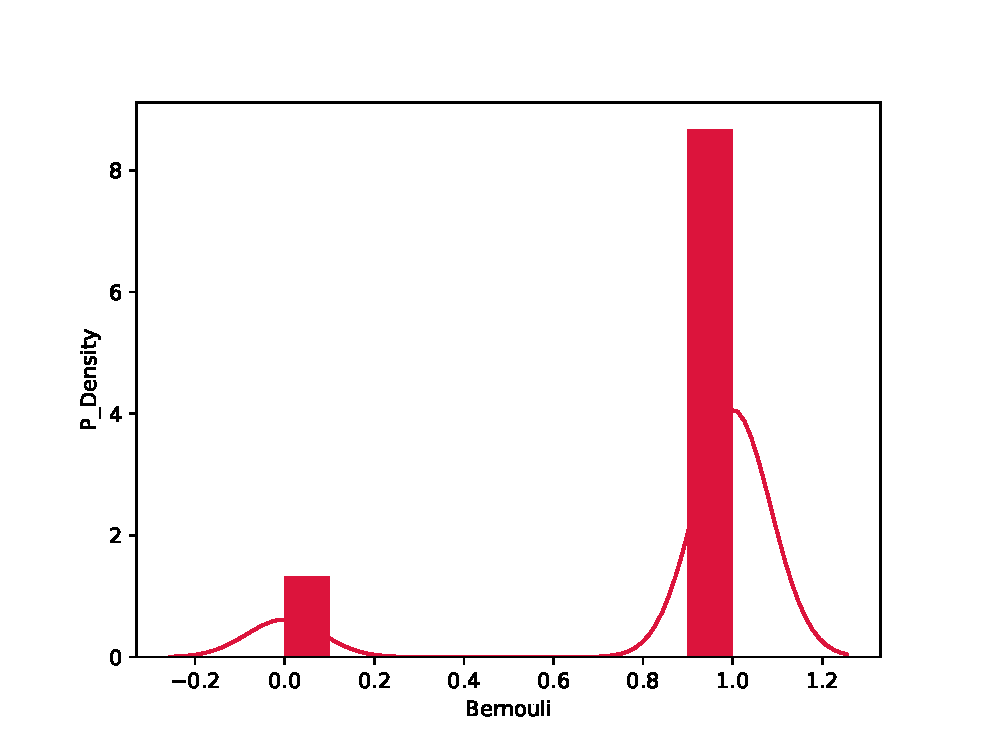
\includegraphics[width=\columnwidth]{./prob/figs/prob2_a.eps}
\caption{Bernoulli Distribution.}
\label{fig:figure1}
\end{figure}
\\
The Bernoulli Distribution of data is given below
\\
Probability mass function(P(X))=$p^x\brak{1-p}^{1-x}$
\begin{align}
P(X=0)=1-p
\\
P(X=1)=p
\end{align}
where p is the probability of occurence of (X=1)
\\
$\therefore$ p=0.861 given by \ref{eq:prob}
\end{enumerate}
\item
The sample size = Total number of pens(S)=
\begin{align}
S=144
\end{align}
Favourable outcome = Pens not purchased(F2)=
\begin{align}
F2=20 
\end{align}
Probabilty(P) of the pens not purchased by her from the shopkeeper=$\frac{20}{144}$
\\
$\therefore$ P = 0.139
\label{eq:prob2}
\\
The python code for the figure \ref{fig:figure2}
\begin{lstlisting}
prob/codes/prob2_b.py
\end{lstlisting}
shows the Bernouli distribution of data.
\begin{figure}[!ht]
\centering
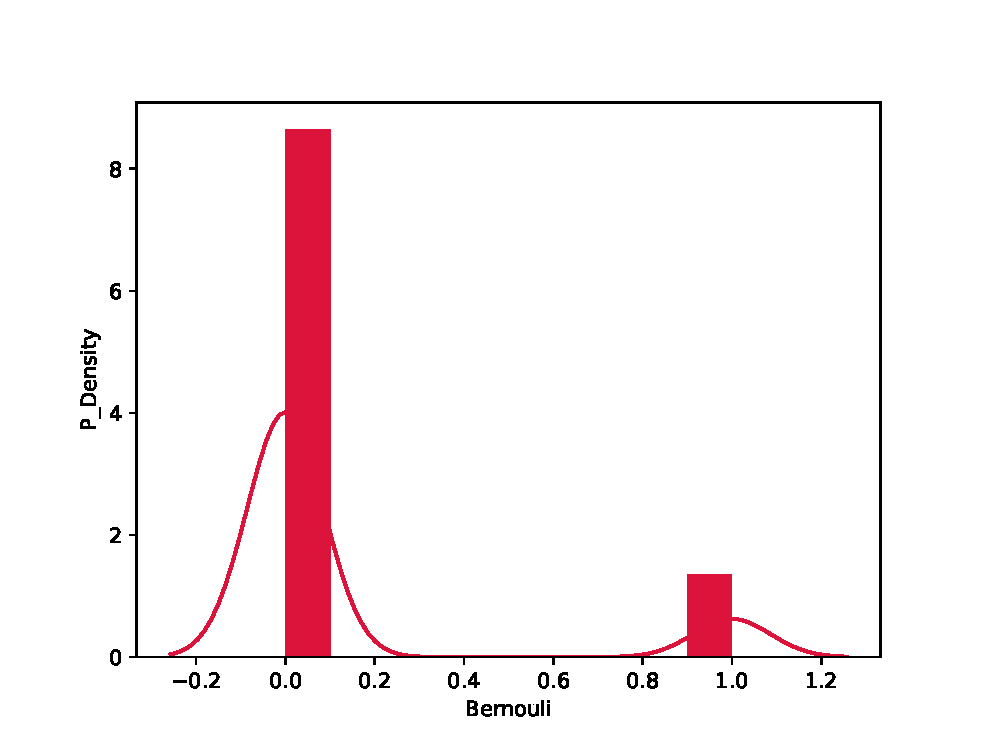
\includegraphics[width=\columnwidth]{./prob/figs/prob2_b.eps}
\caption{Bernoulli Distribution.}
\label{fig:figure2}
\end{figure}
\\
The Bernoulli Distribution of data is given below
\\
Probability mass function(P(X))=$p^x\brak{1-p}^{1-x}$
\begin{align}
P(X=0)=1-p
\\
P(X=1)=p
\end{align}
where p is the probability of occurence of (X=1)
\\
$\therefore$ p=0.139 given by \ref{eq:prob}
\\
The understanding of the curves \ref{fig:figure1} and \ref{fig:figure2} can be seen in \eqref{understandingcurve}
\end{enumerate}